\chapter{Introduzione}
\section{Che cos'è il Brute Force}
Nella crittografia , un attacco di Brute Force consiste in un utente malintenzionato che invia molte password con la speranza di indovinare una combinazione correttamente.

L'aggressore controlla sistematicamente tutte le possibili password finché non trova quella corretta. In alternativa, l'attaccante può tentare di indovinare la chiave che in genere viene creata dalla password utilizzando una funzione di derivazione della chiave.
\begin{figure}[h]
    \centering
    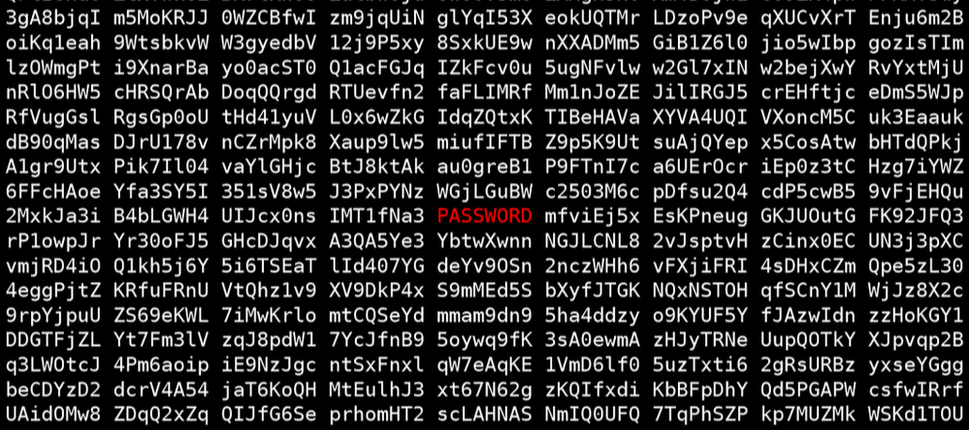
\includegraphics[width=115mm]{Immagini/introduzione/banner.png}
\end{figure}

Un attacco di Brute Force è un attacco crittoanalitico che, in teoria, può essere utilizzato per tentare di decrittografare qualsiasi dato crittografato. Tale attacco potrebbe essere utilizzato quando non è possibile sfruttare altri punti deboli in un sistema di crittografia che renderebbero il compito più semplice.

Gli attacchi di forza bruta funzionano calcolando ogni possibile combinazione che potrebbe costituire una password e testandola per vedere se è la password corretta. All'aumentare della lunghezza della password, la quantità di tempo e la potenza di calcolo richiesta in media per trovare la password corretta aumenta in modo esponenziale.

Per password più lunghe vengono utilizzati altri metodi come l' attacco del dizionario perché una ricerca a forza bruta richiede troppo tempo. Password e chiavi più lunghe hanno più valori possibili e persino più combinazioni, il che le rende esponenzialmente più difficili da decifrare rispetto a quelle più corte.

Gli attacchi di forza bruta possono essere resi meno efficaci offuscando i dati da codificare, rendendo più difficile per un utente malintenzionato riconoscere quando il codice è stato craccato o costringendo l'aggressore a fare più lavoro per testare ogni ipotesi. Una delle misure della forza di un sistema di crittografia è il tempo che teoricamente impiegherebbe un utente malintenzionato per sferrare un attacco di forza bruta riuscito contro di esso.
\section{Hash}
Le funzioni hash \cite{hash} sono particolari funzioni che permettono di dare a un messaggio un’impronta digitale tale da identificarlo univocamente.
\begin{figure}[h]
    \centering
    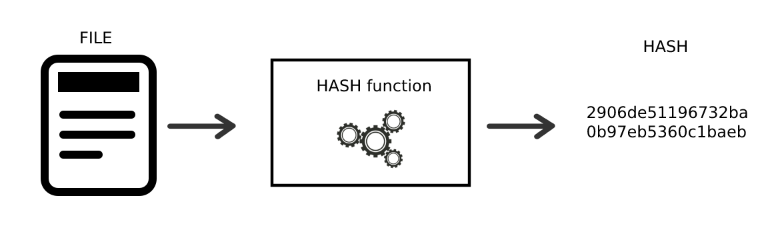
\includegraphics[width=115mm]{Immagini/introduzione/hash.png}
    \label{fig:hash}
\end{figure}

In altre parole creano una stringa associata al messaggio da spedire e per il quale, una volta applicata la funzione, non dovrebbe essere più possibile ritornare al testo originale.
Un valore hash \(h\) viene generato da una funzione A con la seguente forma :
\[ h = H(M)\]
dove M è un messaggio di lunghezza variabile e H(M) è un valore hash di lunghezza fissa.
Lo scopo di una funzione hash è quello di produrre una sorta di "impronta digitale" di un file, messaggio o blocco di dati. Per poter essere utile per l'autenticazione dei messaggi, una funzione hash H deve avere le seguenti proprietà.
\begin{enumerate}
    \item H può essere applicata a un blocco di di dati di qualsiasi dimensione.
    \item H produce un output di lunghezza fissa.
    \item Per un determinato valore \(h\) è computazionalmente impossibile trovare \(x\) tale che \(H(x)\). In generale questa proprietà è detta \textbf{monodirezionalità}.
    \item Per un determinato blocco \(x\) è computazionalmente impossibile trovare \(y \neq x\) tale che \(H(y) = H(x)\). Questa proprietà è chiamata \textbf{resistenza debole alle collisioni}.
    \item È computazionalmente impossibile trovare una coppia \((x, y)\) tale che \(H(x) = H(y)\). Questa viene chiamata \textbf{resistenza forte alle collisioni}.
\end{enumerate}

Il terzo punto, ci indica che è facile generare un codice sulla base di un messaggio, mentre è praticamente impossibile generare impossibile generare un messaggio sulla base di un codice. Questa proprietà è importante se la tecnica di autenticazione prevede l'uso di un valore segreto. Il valore segreto non viene però inviato; al contrario se la funzione hash non fosse monodirezionale, un estraneo con in mano sia il valore segreto che l'hash generato \(C = H(S\ped{AB} \| M)\), sarebbe in grado di invertire l'operazione. Poiché ha sia \(M\) che \(S\ped{AB} \| M\), potrà ricuperare \(S\ped{AB}\).

Tutte le funzioni hash utilizzano i seguenti principi generali. L'input viene elaborato un blocco alla volta in modo iterativo per produrre una funzione hash di \(n\) bit.

Una delle funzioni hash più semplici è una operazione di OR esclusivo bit a bit (XOR) applicata a ciascun blocco.
\[ C\ped{i} = b\ped{i1} \oplus b\ped{i2} \oplus ... \oplus b\ped{im}\]
\newline
dove : 

\begin{itemize}
    \item \(C\ped{i}\) = i-esimo bit del codice hash, \(1 \leq i \leq n\).
    \item m = numero di blocchi di \(n\) bit di input.
    \item b\ped{ij} = i-esimo bit nel j-esimo blocco.
    \item \(\oplus\) = operazione XOR.
\end{itemize}

\begin{table}[htbp]
    \begin{center}

    \begin{tabular}{|l|l|l|l|l|}
        \hline
                    & Bit 1                     & Bit 2                     & ...                       & Bit \(n\)                 \\
                    \hline
        Blocco 1    & b\ped{11}                 & b\ped{21}                 &                           & b\ped{n1}                 \\
        \hline
        Blocco 2    & b\ped{12}                 & b\ped{22}                 &                           & b\ped{n2}                 \\
        \hline
                    & \begin{tabular}[c]{@{}l@{}}.\\ .\\ .\end{tabular} & \begin{tabular}[c]{@{}l@{}}.\\ .\\ .\end{tabular} & \begin{tabular}[c]{@{}l@{}}.\\ .\\ .\end{tabular} & \begin{tabular}[c]{@{}l@{}}.\\ .\\ .\end{tabular} \\
        \hline
        Blocco m    & b\ped{1m}                 & b\ped{2m}                 &                           & b\ped{nm}                 \\
        \hline
        Codice hash & C\ped{1}                  & C\ped{2}                  &                           & C\ped{n} \\
        \hline
    \end{tabular}
\end{center}
\caption{semplice funzione hash con utilizzo di XOR bit a bit.}
\end{table}

\subsection{Types}
Le principali funzioni hash presenti attualmente sono:
\begin{itemize}
    \item \textbf{MD2}\newline  acronimo di Message Digest Algorithm, produce un valore hash di 128 bit e richiede come input multipli di 16 byte. La funzione, inoltre, usa un padding, cioè aggiunge dei bit mancanti ai messaggi in input che non hanno la lunghezza giusta. Questo algoritmo è già stato violato.
    \item \textbf{MD4}\newline anche questa funzione usa hash a 128 bit, ma è più veloce di MD2. Processa il messaggio dividendolo in blocchi di 512 bit. Il padding del messaggio, inoltre, comprende un valore di 64 bit che indica la lunghezza del messaggio originale. Questa funzione è più sicura della precedente, in quanto la difficoltà di produrre due messaggi che hanno la stessa lunghezza con modulo \(2^{64}\) è maggiore.
    \item \textbf{MD5}\newline è stato ideato dopo la violazione di MD4, su cui è basato. Il testo è diviso in blocchi 512 bit e viene generato un hash di 128 bit. E’ basato su XOR e operazioni logiche. L’unico svantaggio è dovuto dal fatto che è un po’ più lento di MD4.
    \item \textbf{SHA-1}\newline  acronimo di Secure Hash Algorithm-1 (anche SHS, Secure Hash Standard), sviluppato dal NSA su richiesta del NIST (National Institute of Standard and Technology). Utilizza gli stessi principi di MD4 e MD5. Il progetto originale del 1994 aveva il nome di SHA, poi modificato nel codice dal NSA. Produce output di 160 bit a partire da una lunghezza arbitraria. Attualmente è uno dei più sicuri, usato anche dai servizi PGP e GPG per firmare documenti.
    \item \textbf{SHA-2}\newline versione successiva a SHA-1, genera impronte di documenti da 256, 384 e 512 bit.
\end{itemize}
\section{Password analysis}
Una cosa da conoscere per effettuare un buon attacco di Brute Force, è la composizione di una password e la sua tassonomia \cite{hashcrack}, da uno studio generale delle password è stato notato che :
\begin{itemize}
    \item la lunghezza media di una password è di 7 - 9 caratteri
    \item si ha il 50\% di possibilità che una password contenga una o più vocali
    \item le donne preferiscono utilizzare nomi per le loro password e gli uomini preferiscono gli hobby
    \item i simboli più utilizzati sono : \textasciitilde, !, @, \#, \$, \%, \&, *, e ?
    \item se si utilizza un numero è il 1 o il 2 e sono utilizzati alla fine
    \item se si utilizza più di un numero, sono sequenze o numeri personali
    \item se si utilizza una lettere maiuscola, questa si trova all'inizio
    \item 66\% delle persone utilizza 1-3 password per tutti i suoi account
    \item una persona su nove ha una password basata sulle 500 password più utilizzate
    \item i paesi occidentali preferiscono le password in minuscolo e i paesi dell'est preferiscono le cifre
\end{itemize}

Le password possono contenere molte informazioni al riguardo al suo creatore, molte volte la stessa persona utilizza un pattern specifico per la creazione delle proprie password, dove andrà a cambiare piccoli dettagli tra una password e l'altra.
Questi pattern si possono suddividere in :
\begin{itemize}
    \item \textbf{Basic Pattern}\newline
          Visibile facilmente, composto da gruppi ben distinti\newline
          \begin{figure}[h]
              \centering
              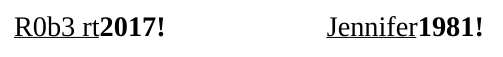
\includegraphics[width=\linewidth]{Immagini/introduzione/Basic_Pattern.png}
              \caption{Basic Pattern}
              \label{fig:basic}
          \end{figure}
          \newline Qui possiamo notare che ogni password è composta da un nome e termina con quattro numeri con lo stesso carattere speciale \!.
    \item \textbf{Macro Pattern}\newline
          Statiche sulla struttura come lunghezza e set di caratteri\newline
          \begin{figure}[h]
              \centering
              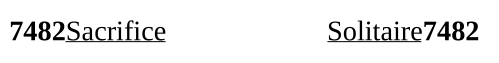
\includegraphics[width=\linewidth]{Immagini/introduzione/Macro_pattern.png}
              \caption{Macro Pattern}
              \label{fig:macro}
          \end{figure}
          \newline Qui possiamo notare che le password hanno un loro schema, composto dalla combinazione di 4 numeri e 7 lettere, inoltre la parola inizia in entrambi i casi con una maiuscola ed in entrambi i casi abbiamo sempre la stessa lettere e lo stesso gruppo di numeri.
    \item \textbf{Micro Pattern}\newline
          Utilizzo di temi e dati/interesse personali per la loro composizione\newline
          \begin{figure}[h]
              \centering
              \includegraphics[width=\linewidth]{Immagini/introduzione/Micro_Pattern.png}
              \caption{Micro Pattern}
              \label{fig:micro}
          \end{figure}
          \newline Qui possiamo notare che ogni password inizia con un colore, inoltre la seconda parte è composta da un nome di un animale e si utilizzano 3 numeri diversi per concludere la password.
\end{itemize}

L'individuazione di queste schemi possono andare a ridurre di molto i tempi che si impiegano per trovare le password, perché ci permettono di capire quale tecnica è più adeguata da applicare e quali regole applicare per l’esecuzione dell’attacco.

\subsection{20-60-20 RULE}

La regola 20-60-20 è un modo per visualizzare il livello di distribuzione delle password in base alla loro complessità, con caratteristiche che generalmente seguono quelle di una curva gaussiana, dove sull'asse delle X abbiamo la complessità della password e sul lato delle Y abbiamo il "numero" di quante persone la utilizzano.
\begin{itemize}
    \item Il 20\% delle password sono parole del dizionario facilmente indovinabili o password comuni.
    \item Il 60\% delle password sono variazioni da moderate a leggere rispetto al precedente 20\%.
    \item Il 20\% delle password sono rigide, lunghe, complesse o con caratteristiche uniche.
\end{itemize}

\newpage

\begin{figure}[htpb!]
    \centering
    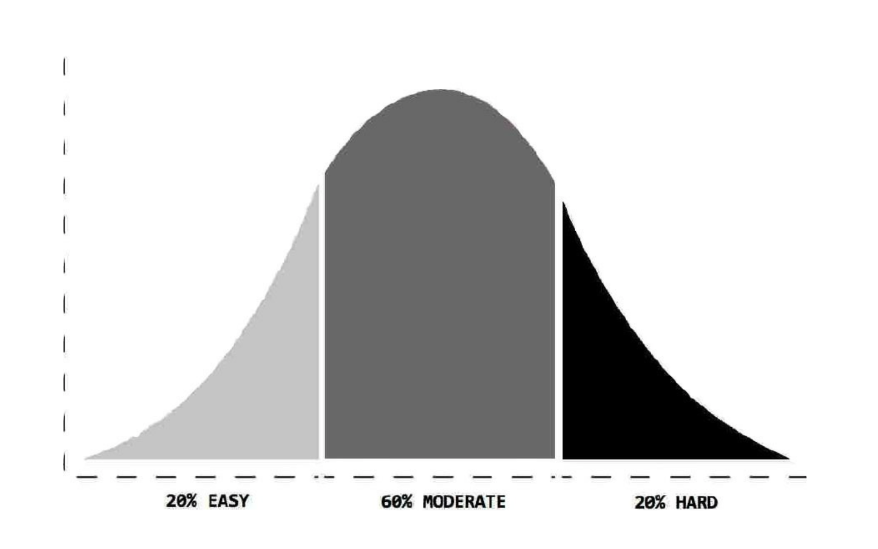
\includegraphics[width=\linewidth]{Immagini/introduzione/20-60-20.png}
    \caption{Rule 20-60-20 \cite{hashcrack}}
    \label{fig:rocker}
\end{figure}

\section{Strumenti}

Per eseguire il brute force, possiamo trovare moltissimi tool nel web, ma ci sono due programmi che spuntano tra di questi, per la loro efficacia e per la loro flessibilità nel permettere di eseguire diversi tipi di attacchi.

\subsection{John The Ripper}

\begin{figure}[htpb!]
    \centering
    
\includegraphics[width=60mm]{Immagini/1/john.png}
    \caption{John The Ripper logo}
\end{figure}

John the Ripper \cite{John_The_Ripper} è un software per craccare password che inizialmente era disponibile solo su UNIX. Solo dal 2012 è stato possibile eseguirlo su 15 piattaforme diverse, tra cui Windows.

Il programma combina diverse modalità di rottura in un unico programma ed è completamente configurabile in base alle proprie necessità.
\newpage
Le tipologie di attacchi che possiamo eseguire con questo strumento sono :
\begin{itemize}
    \item Bruteforce Attack \newline
          \begin{lstlisting}[caption={John the ripper Bruteforce}, style=javaScriptCode]
        john --format=#type hash.txt
    \end{lstlisting}
    \item Dictionary Attack \newline
          \begin{lstlisting}[caption={John the ripper Dictionary}, style=javaScriptCode]
        john --format=#type --wordlist=dict.txt hash.txt
    \end{lstlisting}
    \item Mask Attack \newline
          \begin{lstlisting}[caption={John the ripper Mask}, style=javaScriptCode]
        john --format=#type --mask=?l?l?l?l?l?l -min-len=6
    \end{lstlisting}
    \item Incremental Attack \newline
          \begin{lstlisting}[caption={John the ripper Incremental}, style=javaScriptCode]
        john --incremental hash.txt
    \end{lstlisting}
    \item Dictionary + Rule Attack \newline
          In aggiunta al Dictionary attack possiamo applicare delle regole, queste regole vengono inserite tramite il comando \textbf{--rules=??}.\newline
          Questi regole sono :
          \begin{itemize}
              \item[$\square$] \textbf{--rules=Single}
              \item[$\square$] \textbf{--rules=Wordlist}
              \item[$\square$] \textbf{--rules=Extra}
              \item[$\square$] \textbf{--rules=Jumbo}
              \item[$\square$] \textbf{--rules=KoreLogic}
              \item[$\square$] \textbf{--rules=All}
          \end{itemize}
          \begin{lstlisting}[caption={John the ripper Dictionary + Rule }, style=javaScriptCode]
        john --format=#type --wordlist=dict.txt --rules
    \end{lstlisting}
\end{itemize}

Un'altra funziona di John The Ripper è quella di utilizzare le CPU in parallelo, questo è possibile tramite l'utilizzo del comando :

\begin{lstlisting}[caption={John the ripper Multi-CPU example 8 core}, style=javaScriptCode]
    john --wordlist=dict.txt hash.txt --rules --dev=<#> --fork=8
\end{lstlisting}

Inoltre è possibile eseguire John The Ripper sfruttando la GPU con il comando 
\begin{lstlisting}[caption={John the ripper GPU example}, style=javaScriptCode]
    john --list=formats --format=cuda #for CUDA
    john --list=formats --format=opencl #for Opencl\end{lstlisting}
\subsection{Hashcat}

\begin{figure}[htpb!]
    \centering
    
\includegraphics[width=\linewidth]{Immagini/1/hashcat-logo.png}
    \caption{Hashcat logo}
\end{figure}

Hashcat \cite{hashcat} è l'utility di recupero password più veloce e avanzata al mondo, che supporta sei modalità di attacco uniche per oltre 300 algoritmi di hashing altamente ottimizzati. hashcat attualmente supporta CPU, GPU e altri acceleratori hardware su Linux, Windows e macOS e dispone di strutture per consentire il cracking distribuito delle password.

I tipi di attacchi supportati sono :
\begin{itemize}
    \item Brute Force
          \begin{lstlisting}[caption={Hashcat Brute Force}, style=javaScriptCode]
        hashcat -a 3 -m #type hash.txt 
    \end{lstlisting}
    \item Dictionary Attack
          \begin{lstlisting}[caption={Hashcat Dictionary}, style=javaScriptCode]
        hashcat -a 0 -m #type hash.txt dict.txt 
    \end{lstlisting}
    \item Combination
          \begin{lstlisting}[caption={Hashcat Combination}, style=javaScriptCode]
        hashcat -a 1 -m #type hash.txt dict1.txt dict2.txt
    \end{lstlisting}
    \item Mask Attack
          \begin{lstlisting}[caption={Hashcat Mask}, style=javaScriptCode]
        hashcat -a 3 -m #type hash.txt ?a?a?a?a?a?a?a?a
    \end{lstlisting}
    \item Hybrid Dictionary + Mask
          \begin{lstlisting}[caption={Hashcat Hybrid Dictionary + Mask}, style=javaScriptCode]
        hashcat -a 6 -m #type hash.txt dict.txt ?a?a?a?a?a?a?a?a
    \end{lstlisting}
    \item Hybrid Mask + Wordlist
          \begin{lstlisting}[caption={Hashcat Hybrid Mask + Wordlist}, style=javaScriptCode]
        hashcat -a 6 -m #type hash.txt ?a?a?a?a?a?a?a?a dict.txt
    \end{lstlisting}
\end{itemize}

Esempio di un Brute Force con Hashcat 

\begin{figure}[h!]
    \centering
    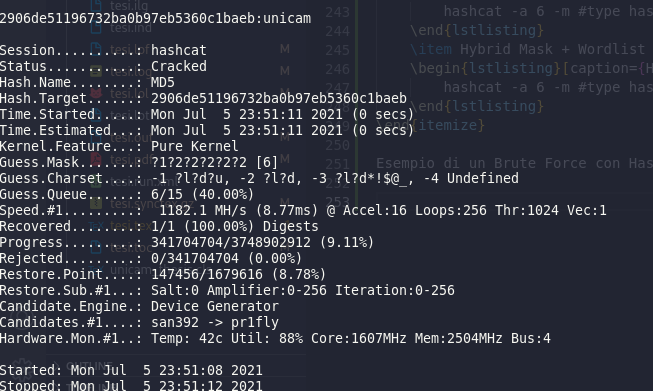
\includegraphics[width=\linewidth]{Immagini/1/hashcat_show.png}
    \caption{hashcat example}
    \label{fig:hashcat example}
\end{figure}

